\chapter{Graphing Motion}

	\section{Introduction}
	Creating graphs of an object's motion is a useful tool for several reasons.  Graphs do all the of the following:
	\begin{itemize}
		\item Graphs allow us to visualize relationships within collected data.
		\item Graphs allow for detailed analysis, allowing us to find regression lines, slope, and area.
		\item Graphs allow for easy and intuitive extrapolation - that is, prediction of future behavior.
		\item Graphs help us to understand complex forms of motion.
		\item Graphs help us to compare different types of motion.
	\end{itemize}

In general, there are three types of graphs that physicists use routinely when studying motion of objects: \textit{Position vs Time graphs, Velocity vs Time graphs,} and \textit{Acceleration vs Time} graphs.  Using each of these types of graph, we will analyze the characteristics of different types of motion.

It may be helpful to review some math.  The formula for a line, in \gls{slopeinterceptformat} is given by:
\begin{mdframed}[backgroundcolor=orange!20!white]
\begin{equation}
	y = m x +b
\end{equation}
\end{mdframed}

where $m$ is the \gls{slope} of the line and $b$ is the \gls{yintercept}.

To determine the slope of a line, use the slope formula: 
\begin{mdframed}[backgroundcolor=orange!20!white]
	\index{Slope}
	\begin{equation}
		m = \frac{rise}{run} = \frac{\Delta y} {\Delta x} = \frac{y_2-y_1}{x_2-x_1}
	\end{equation}
\end{mdframed}


\newpage
	\section{Position vs Time Graphs}
	There are some important things to know about position vs time graphs:
	\begin{itemize}
		\item The slope of a position vs time graph is equal to the object's velocity. 
		\item Curves on a position-time graph indicate acceleration.
	\end{itemize}
With these ideas in mind, let us examine several common types of motion.  

		\subsection{Constant Position}
		An object with a constant position will be at rest; it is not moving.  Thus, a position-time graph for a non-moving object might look something like this: 
		\begin{figure}[h]
			\centering
			\caption{Position-Time Graph for an Object at Rest}
		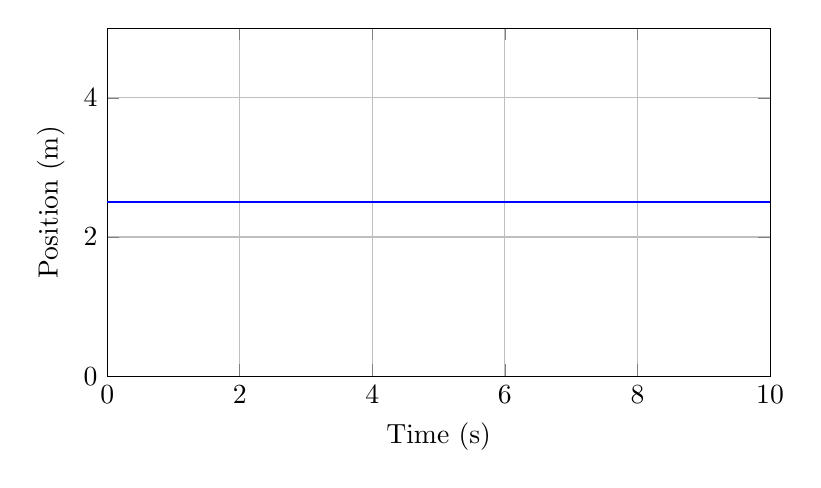
\begin{tikzpicture}
			\begin{axis}[
				xlabel={Time (s)},
				ylabel={Position (m)},
				grid=major,
				%title={Position-Time Graph for an Object at Rest},
				ymin=0, ymax=5, % Adjust the y-axis limits to show position clearly
				xmin=0, xmax=10, % Adjust the x-axis limits for the time range
				width=10cm,
				height=6cm
				]
				% Plot a horizontal line at position = 2.5 meters
				\addplot [domain=0:10, samples=100, thick, blue] {2.5};
				%\addlegendentry{$s(t) = 2.5 \text{ m}$}
			\end{axis}
		\end{tikzpicture}
		\end{figure}
	
		
		\subsection{Constant Velocity}
		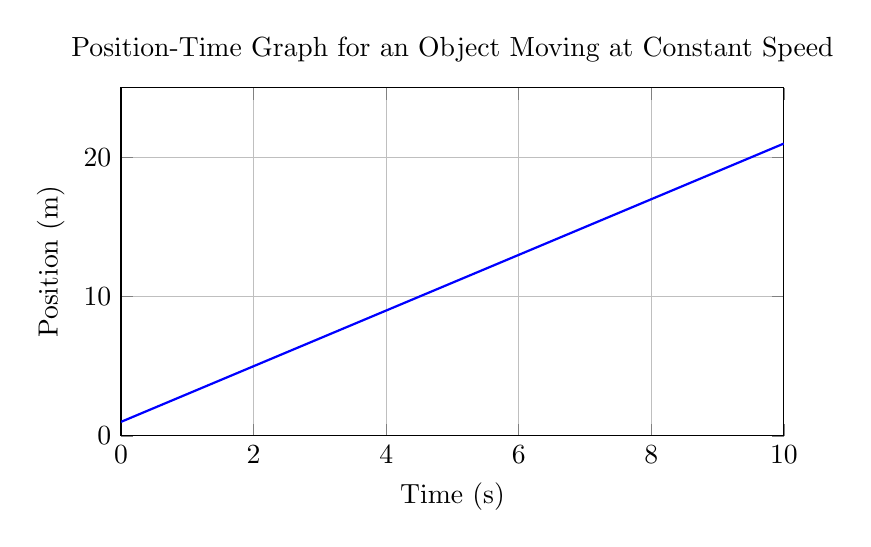
\begin{tikzpicture}
			\begin{axis}[
				xlabel={Time (s)},
				ylabel={Position (m)},
				grid=major,
				title={Position-Time Graph for an Object Moving at Constant Speed},
				ymin=0, ymax=25, % Adjust the y-axis limits to show position clearly
				xmin=0, xmax=10, % Adjust the x-axis limits for the time range
				width=10cm,
				height=6cm
				]
				% Plot the linear function for position: s(t) = 1 + 2t
				\addplot [domain=0:10, samples=100, thick, blue] {1 + 2*x};
			%	\addlegendentry{$s(t) = 1 + 2t$}
			\end{axis}
		\end{tikzpicture}
		
		
		
		
		
		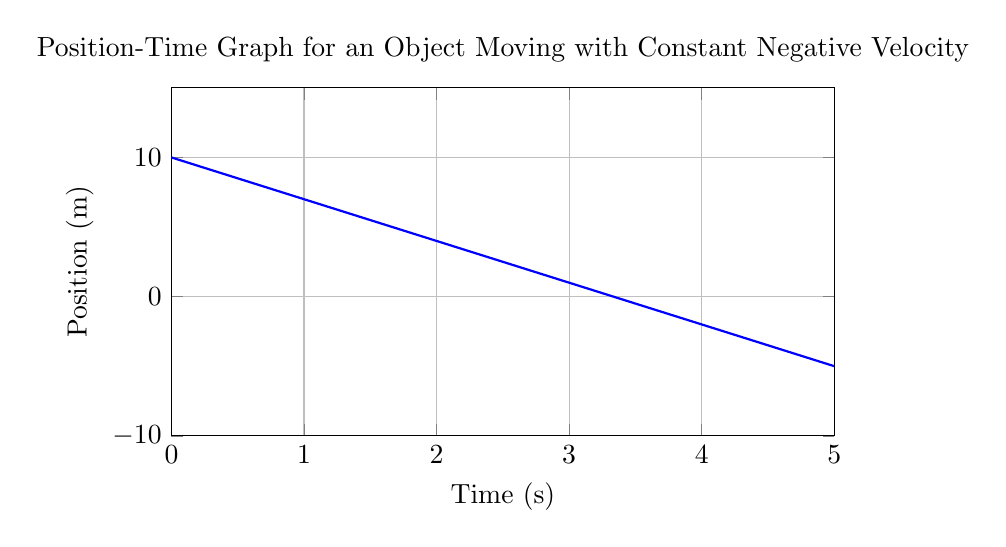
\begin{tikzpicture}
			\begin{axis}[
				xlabel={Time (s)},
				ylabel={Position (m)},
				grid=major,
				title={Position-Time Graph for an Object Moving with Constant Negative Velocity},
				ymin=-10, ymax=15, % Adjust the y-axis limits to show position clearly
				xmin=0, xmax=5, % Adjust the x-axis limits for the time range
				width=10cm,
				height=6cm
				]
				% Plot the linear function for position: s(t) = 10 - 3t
				\addplot [domain=0:5, samples=100, thick, blue] {10 - 3*x};
			%	\addlegendentry{$s(t) = 10 - 3t$}
				
				% Mark the starting point (0, 10)
			%	\addplot[mark=*] coordinates {(0, 10)};
			%	\node at (0, 10) [above right] {Start};
				
				% Mark the ending point (5, -5)
			%	\addplot[mark=*] coordinates {(5, -5)};
			%	\node at (5, -5) [below left] {End};
				
			\end{axis}
		\end{tikzpicture}
	
	
		
		\subsection{Constant Acceleration}
		
		
		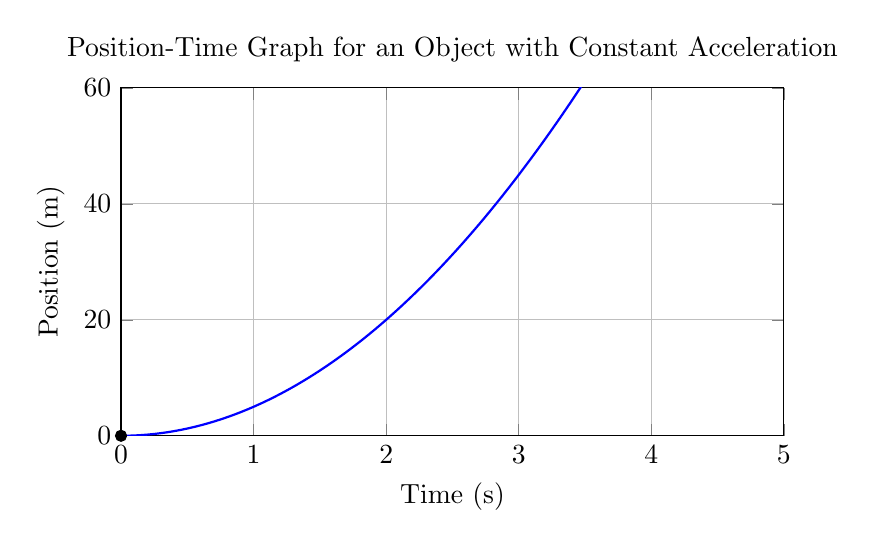
\begin{tikzpicture}
			\begin{axis}[
				xlabel={Time (s)},
				ylabel={Position (m)},
				grid=major,
				title={Position-Time Graph for an Object with Constant Acceleration},
				ymin=0, ymax=60, % Adjust the y-axis limits to show position clearly
				xmin=0, xmax=5, % Adjust the x-axis limits for the time range
				width=10cm,
				height=6cm
				]
				% Plot the quadratic function for position: s(t) = 5t^2
				\addplot [domain=0:5, samples=100, thick, blue] {5*x^2};
			%	\addlegendentry{$s(t) = 5t^2$}
				
				% Mark the origin point (0, 0)
				\addplot[mark=*] coordinates {(0, 0)};
				\node at (0, 0) [below right] {Start};
				
			\end{axis}
		\end{tikzpicture}
		
		
		
	\section{Velocity vs Time Graphs}
	
<<<<<<< Updated upstream
	Velocity vs Time graphs have different properties than position vs time graphs.  Important characteristics of this type of graph include:
	\begin{itemize}
		\item The slope of a velocity vs time graph is the acceleration of the object.
		\item The distance traveled by an object is given by the area under the line or curve.
	\end{itemize}
	
		\subsection{Constant Position}
		
		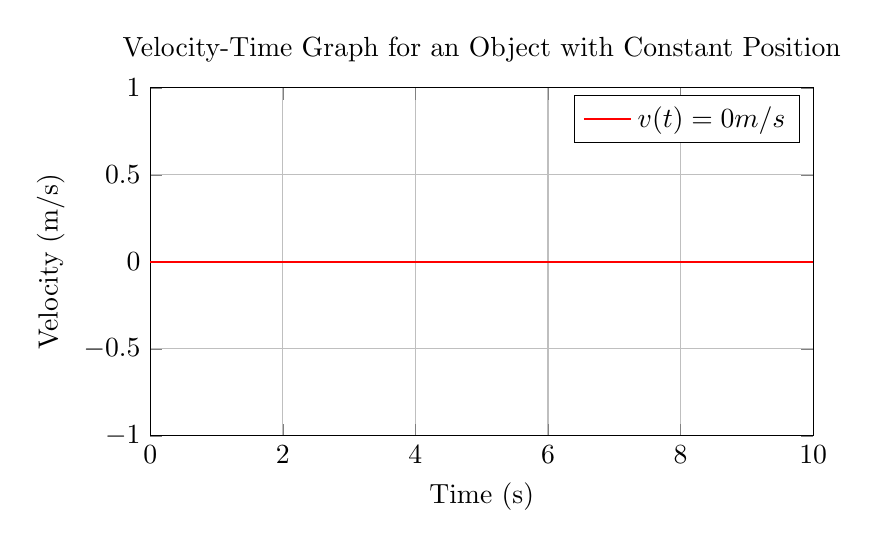
\begin{tikzpicture}
		\begin{axis}[
		xlabel={Time (s)},
		ylabel={Velocity (m/s)},
		grid=major,
		title={Velocity-Time Graph for an Object with Constant Position},
		ymin=-1, ymax=1, % Adjust the y-axis limits to show velocity clearly
		xmin=0, xmax=10, % Adjust the x-axis limits for the time range
		width=10cm,
		height=6cm
		]
		% Plot a constant velocity of 0 m/s
		\addplot [domain=0:10, samples=100, thick, red] {0};
		\addlegendentry{$v(t) = 0 \text{ m/s}$}
		
		% Mark the velocity line with a label
		\node at (0, 0) [left] {Zero Velocity};
		
		\end{axis}
		\end{tikzpicture}
=======
	
		\subsection{Constant Position}
		
		

			
			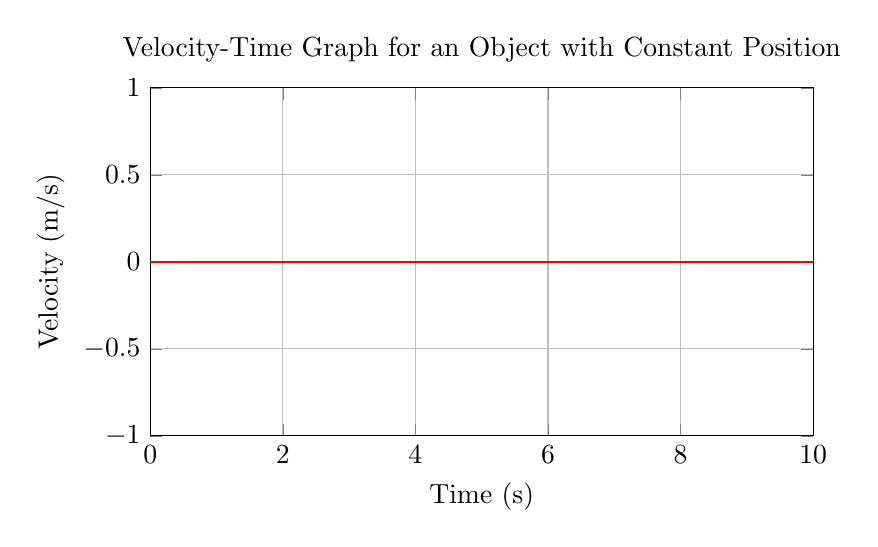
\begin{tikzpicture}
				\begin{axis}[
					xlabel={Time (s)},
					ylabel={Velocity (m/s)},
					grid=major,
					title={Velocity-Time Graph for an Object with Constant Position},
					ymin=-1, ymax=1, % Adjust the y-axis limits to show velocity clearly
					xmin=0, xmax=10, % Adjust the x-axis limits for the time range
					width=10cm,
					height=6cm
					]
					% Plot a constant velocity of 0 m/s
					\addplot [domain=0:10, samples=100, thick, red] {0};

					
					% Mark the velocity line with a label
					\node at (0, 0) [left] {Zero Velocity};
					
				\end{axis}
			\end{tikzpicture}
			

>>>>>>> Stashed changes
		
		
		
		\subsection{Constant Velocity}
		
		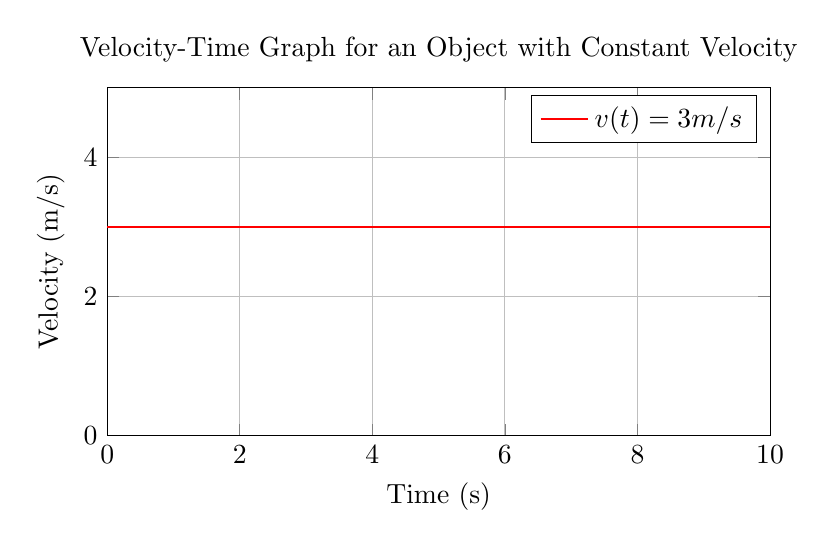
\begin{tikzpicture}
<<<<<<< Updated upstream
		\begin{axis}[
		xlabel={Time (s)},
		ylabel={Velocity (m/s)},
		grid=major,
		title={Velocity-Time Graph for an Object with Constant Velocity},
		ymin=0, ymax=5, % Adjust the y-axis limits to show velocity clearly
		xmin=0, xmax=10, % Adjust the x-axis limits for the time range
		width=10cm,
		height=6cm
		]
		% Plot a constant velocity of 3 m/s
		\addplot [domain=0:10, samples=100, thick, red] {3};
		\addlegendentry{$v(t) = 3 \text{ m/s}$}
		
		% Mark the velocity line with a label
		\node at (0, 3) [left] {Constant Velocity};
		
		\end{axis}
		\end{tikzpicture}
		
		\subsection{Constant Acceleration}
		
			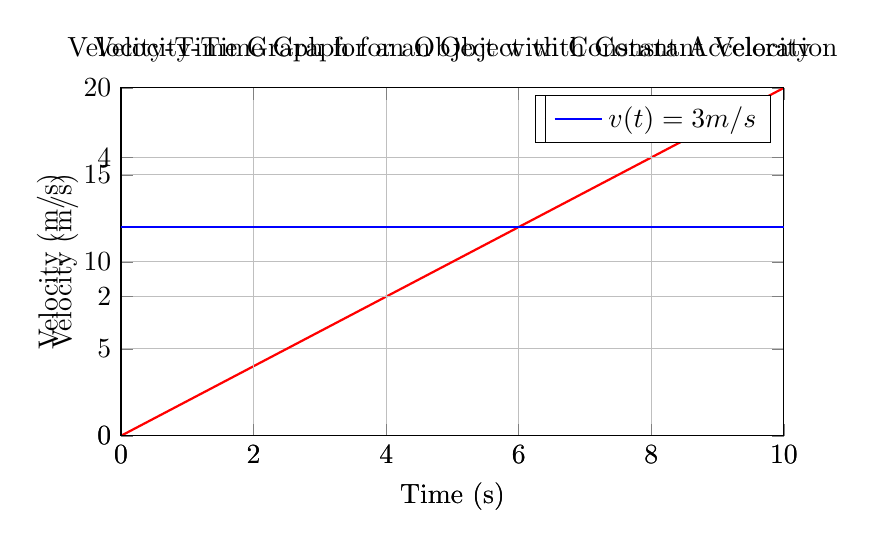
\begin{tikzpicture}
		\begin{axis}[
		xlabel={Time (s)},
		ylabel={Velocity (m/s)},
		grid=major,
		title={Velocity-Time Graph for an Object with Constant Acceleration},
		ymin=0, ymax=20, % Adjust the y-axis limits to show velocity clearly
		xmin=0, xmax=10, % Adjust the x-axis limits for the time range
		width=10cm,
		height=6cm
		]
		% Plot a linear velocity function with constant acceleration, v(t) = 2t
		\addplot [domain=0:10, samples=100, thick, red] {2*x};
		\addlegendentry{$v(t) = 2t \text{ m/s}$}
		
		% Mark the initial point with a label
		\node at (0, 0) [below right] {Start};
		
		\end{axis}
=======
			\begin{axis}[
				xlabel={Time (s)},
				ylabel={Velocity (m/s)},
				grid=major,
				title={Velocity-Time Graph for an Object with Constant Velocity},
				ymin=0, ymax=5, % Adjust the y-axis limits to show velocity clearly
				xmin=0, xmax=10, % Adjust the x-axis limits for the time range
				width=10cm,
				height=6cm
				]
				% Plot a constant velocity of 3 m/s
				\addplot [domain=0:10, samples=100, thick, blue] {3};
				\addlegendentry{$v(t) = 3 \text{ m/s}$}
				
				% Mark the velocity line with a label
				\node at (0, 3) [left] {Constant Velocity};
				
			\end{axis}
		\end{tikzpicture}
	
		
		\subsection{Constant Acceleration}
		
		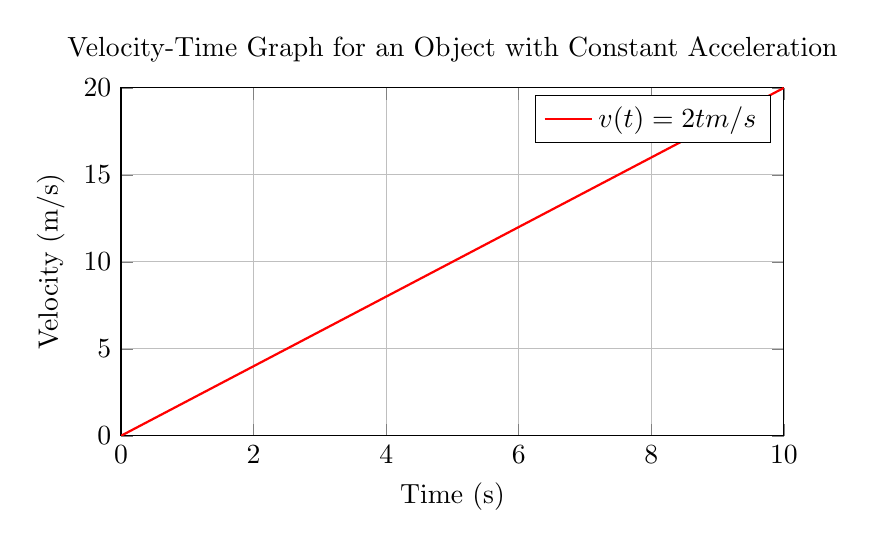
\begin{tikzpicture}
			\begin{axis}[
				xlabel={Time (s)},
				ylabel={Velocity (m/s)},
				grid=major,
				title={Velocity-Time Graph for an Object with Constant Acceleration},
				ymin=0, ymax=20, % Adjust the y-axis limits to show velocity clearly
				xmin=0, xmax=10, % Adjust the x-axis limits for the time range
				width=10cm,
				height=6cm
				]
				% Plot a linear velocity function with constant acceleration, v(t) = 2t
				\addplot [domain=0:10, samples=100, thick, red] {2*x};
				\addlegendentry{$v(t) = 2t \text{ m/s}$}
				
				% Mark the initial point with a label
				\node at (0, 0) [below right] {Start};
				
			\end{axis}
>>>>>>> Stashed changes
		\end{tikzpicture}
		
	\section{Acceleration vs Time Graphs}
	For acceleration vs time graphs,
	\begin{itemize}
		\item The area under the line is equal to the change in velocity.
		\item The slope of the line is called \gls{jerk}, but isn't often used.
	\end{itemize}
	
		\subsection{Constant Position}
		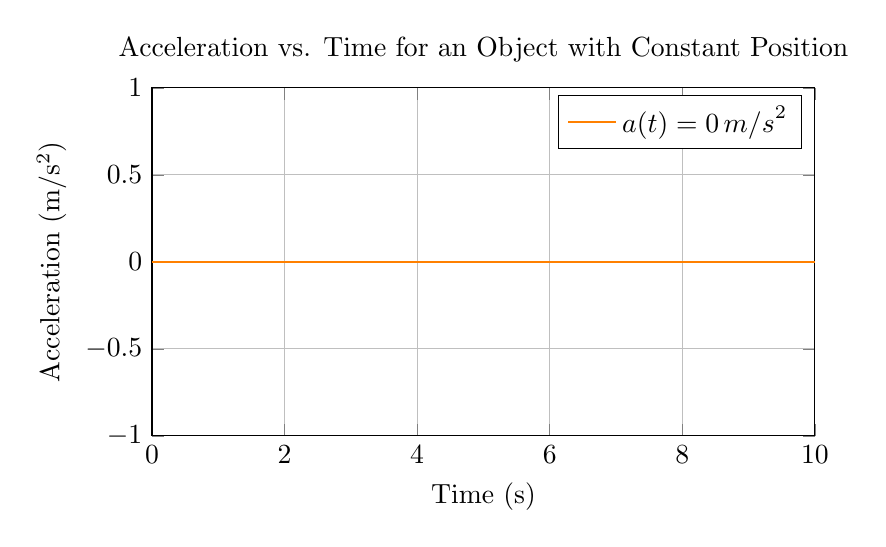
\begin{tikzpicture}
		\begin{axis}[
		xlabel={Time (s)},
		ylabel={Acceleration (m/s\(^2\))},
		grid=major,
		title={Acceleration vs. Time for an Object with Constant Position},
		ymin=-1, ymax=1, % Set y-axis limits to show zero acceleration clearly
		xmin=0, xmax=10, % Set x-axis limits for the time range
		width=10cm,
		height=6cm
		]
		% Plot a constant acceleration of 0 m/s^2
		\addplot [domain=0:10, samples=100, thick, orange] {0};
		\addlegendentry{$a(t) = 0 \, \text{m/s}^2$}
		
		% Mark the zero line with a label
		\node at (0, 0) [left] {0};
		
		\end{axis}
		\end{tikzpicture}
		
		\subsection{Constant Velocity}
		
		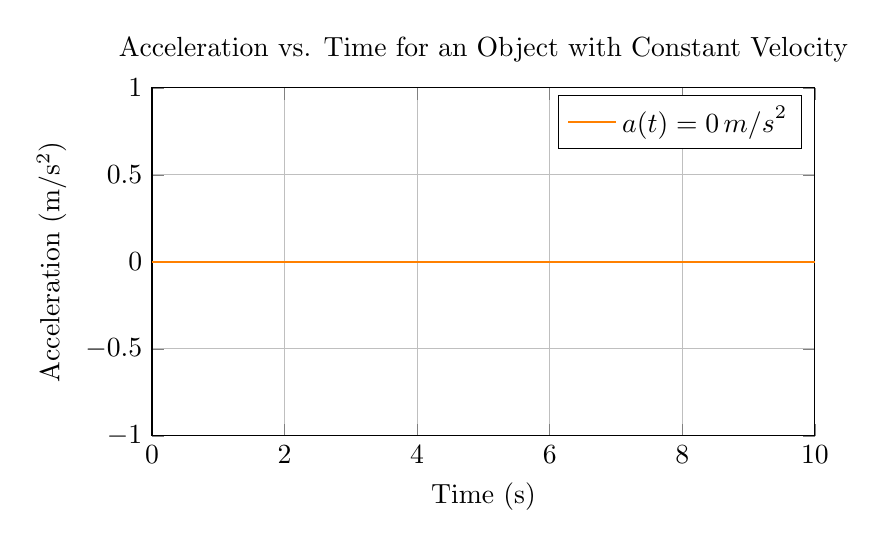
\begin{tikzpicture}
		\begin{axis}[
		xlabel={Time (s)},
		ylabel={Acceleration (m/s\(^2\))},
		grid=major,
		title={Acceleration vs. Time for an Object with Constant Velocity},
		ymin=-1, ymax=1, % Set y-axis limits to show zero acceleration clearly
		xmin=0, xmax=10, % Set x-axis limits for the time range
		width=10cm,
		height=6cm
		]
		% Plot a constant acceleration of 0 m/s^2
		\addplot [domain=0:10, samples=100, thick, orange] {0};
		\addlegendentry{$a(t) = 0 \, \text{m/s}^2$}
		
		% Mark the zero line with a label
		\node at (0, 0) [left] {0};
		
		\end{axis}
		\end{tikzpicture}
		
		\subsection{Constant Acceleration}	
	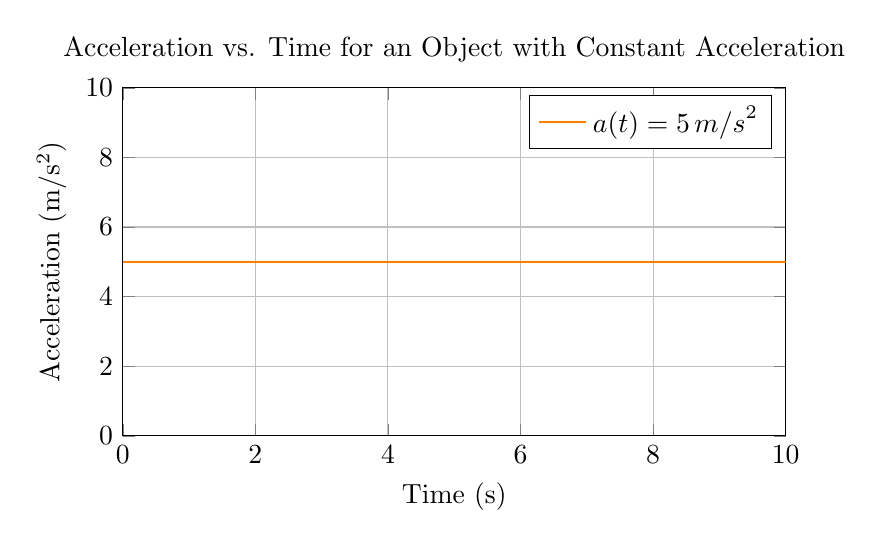
\begin{tikzpicture}
	\begin{axis}[
	xlabel={Time (s)},
	ylabel={Acceleration (m/s\(^2\))},
	grid=major,
	title={Acceleration vs. Time for an Object with Constant Acceleration},
	ymin=0, ymax=10, % Set y-axis limits to show acceleration clearly
	xmin=0, xmax=10, % Set x-axis limits for the time range
	width=10cm,
	height=6cm
	]
	% Plot a constant acceleration of 5 m/s^2 with orange color
	\addplot [domain=0:10, samples=100, thick, orange] {5};
	\addlegendentry{$a(t) = 5 \, \text{m/s}^2$}
	
	% Mark the constant acceleration line with a label
	\node at (0, 5) [left] {5 m/s\(^2\)};
	
	\end{axis}
	\end{tikzpicture}

	


